\section{The Algorithm}
Our approach to this problem is inspired by the observation on how humans
extend a leg or an arm at the appropriate moment to stop a fall. In
this section, we
will describe an abstract model to approximate this behavior, use this
model to plan the optimal sequence of contacts, and finally execute
the plan on the humanoid robots.

% \updated{Human intentionally reaches the ground to absorb the shock with the
%   desired body parts at the right moments, such as taking a step or pushing
%   the ground with arms.
%   We will describe this behavior with an abstract model and plan the optimal
%   contact sequence using this model.}
%% - Human intentionally establish contacts to break a fall, such as
%% taking a step or stick the arm out.
%% - We seek for an abstract model to represent this behavior and plan
%% the contact sequence using this model.

\subsection{Abstract Model}
\begin{figure}[ht]
\center
  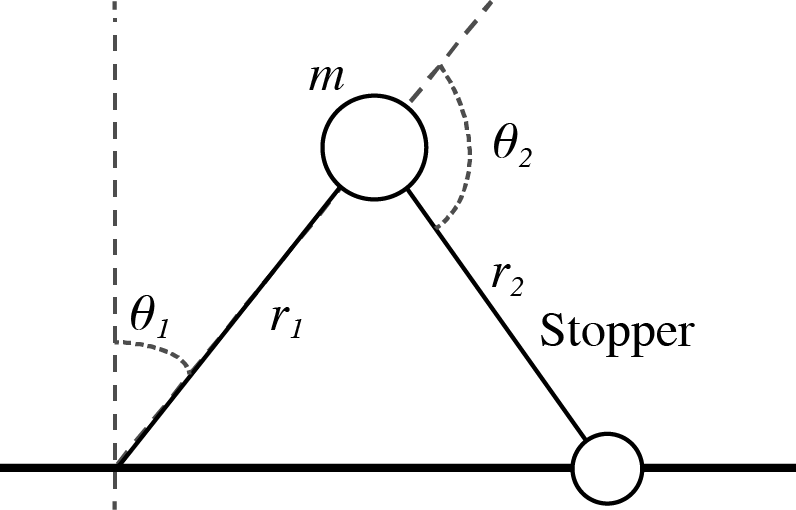
\includegraphics[width=2.5in]{images/tip.png}
  \caption{
    The abstract model consists of a telescopic inverted pendulum and  a massless
      stopper.}
    %% \karen{Replace COM with $m$. Remove the arrow around
    %%   $r_1$. Move ``stopper'' a bit higher as it describes the entire
    %%   stopper not just the tip. Make sure all the math symbols are in
    %%   italic mode to match the format in the text.}
  
  \label{fig:falling_tip}
\end{figure}
The falling motion of biped humanoids has been modelled by a simple 2D
inverted pendulum with a massless telescopic rod
\cite{Fujiwara:2003:FHH,Fujiwara:2006:TOF}. The pivot and the center
of mass (COM) of the pendulum represent the center of pressure (COP)
and the COM of the robot respectively in the sagittal plane. To model
the behavior of breaking a fall using contact, we add an additional
massless telescopic rod, called a stopper, to the standard telescopic
inverted pendulum (\figref{falling_tip}). The configuration of our abstract
model can be defined by the pendulum length ($r_1$), the angle between
the pendulum rod and the vertical line ($\theta_1$), the length of the
stopper ($r_2$), and the angle between the pendulum rod and the
stopper rod ($\theta_2$). We assume that the abstract model has
control over $r_1$, $\theta_2$, $r_2$, but $\theta_1$ is left
unactuated. By controlling these three variables, our goal is to
minimize the vertical impulse at the contact.

Because the stopper is massless, the equations of motion
of the abstract model only depend on $\theta_1$ and $r_1$ and can be
written as:
  \begin{eqnarray}
    r_1 \ddot{\theta}_1 + 2\dot{r}_1\dot{\theta}_1 - g \sin \theta_1
    = 0 
    \label{eq:falling_eom1} \\
    m\ddot{r}_1 - m r_1 \dot{\theta}_1^2 + mg \cos\theta_1 = \tau_{r_1},
    \label{eq:falling_eom2}
  \end{eqnarray}
where $m$ is the mass of the robot and $g$ is the gravitational
constant. The control force $\tau_{r_1}$ is computed based on the
desired velocity of the pendulum rod, $\dot{r}_1^d$:
  \begin{equation}
    \begin{aligned}
      \tau_{r_1}= \frac{m}{h}(\dot{r}_1^d - \dot{r}_1) -
      mr_1 \dot{\theta}_1^2 + mg \cos\theta_1.
    \label{eq:falling_velcon}
    \end{aligned}
  \end{equation}
 %% \karen{assuming $h$ has been defined previously.}

  Though not involved in the equations of motion, the stopper will
  change the momentum of the abstract model whenever it establishes a
  contact with the ground. Let the COM of the pendulum and the tip of
  the stopper be $(x_1, y_1)$ and $(x_2, y_2)$ respectively, with
  respect to the pivot $(0, 0)$.  The momentum due to the vertical
  impulse $j$ generated by the stopper at the contact can be expressed
  as:
  \begin{equation}
    \begin{aligned}
      P_y^+ &= m\dot{y_1}^+ = m\dot{y_1}^- + j \\
      L^+ &=  I\dot{\theta_1}^+ = I\dot{\theta_1}^- - (x_2 - x_1)j,
    \end{aligned}
  \end{equation}
  where $P$ and $L$ are linear and angular momentum of the abstract
  model and $I$ is the estimated inertia. Because we do not know the
  fullbody pose when planning in the space of the abstract model, we
  approximate the inertia using the initial configuration of the robot
  at the beginning of the fall. The superscripts $^-$ and $^+$ denote
  the quantities before and after the impact respectively. For
  inelastic collision, the vertical velocity at the tip of the stopper
  after the impact should be equal to zero, leading to the following
  equation:
  \begin{equation}
    \label{eq:falling_impulse0}
    \begin{aligned}
      0 &= \dot{y}_2^+ = \dot{y}_1^+ - (x_2 - x_1)\dot{\theta}_1^+ \\
      &= (\dot{y}_1^- + \frac{j}{m}) - (x_2 - x_1)(\dot{\theta}_1^- - \frac{(x_2 - x_1)j}{I}) \\
      &= (\frac{1}{m} + \frac{1}{I}(x_2 - x_1)^2) j + \dot{y}_2^-.
    \end{aligned}
  \end{equation}
\eqnref{falling_impulse0} gives a formula to compute the vertical
impulse $j$:
  \begin{equation}
    \begin{aligned}
      j = -\frac{\dot{y}_2^-}{\frac{1}{m} + \frac{1}{I}(x_2 - x_1)^2}.
      \label{eq:falling_impulse1}
    \end{aligned}
  \end{equation}

